\documentclass[]{article}
\usepackage{geometry,tikz,lipsum,amsmath,amssymb,soul,xcolor,cancel}
\usepackage[dvipsnames]{xcolor}
\tikzset{every picture/.style={line width=0.75pt}} %set default line width to 0.75pt        
\numberwithin{equation}{section}

\NewDocumentCommand{\caja}{ m O{gray!40} O{gray!10} m }{
	\begin{figure}[h]
		\centering
		\begin{tikzpicture}
			\node[anchor=text, text width=\columnwidth-1.2cm, draw, rounded corners, line width=1pt, fill=#3, inner sep=5mm] (big) {\\#4};
			\node[draw, rounded corners, line width=.5pt, fill=#2, anchor=west, xshift=5mm] (small) at (big.north west) {#1};
		\end{tikzpicture}
	\end{figure}
}
\NewDocumentCommand{\indUpDown}{ O{\Lambda} O{\mu} O{\nu} }{
	{#1}^{#2}_{\ #3}
}
\NewDocumentCommand{\indDownUp}{ O{\Lambda} O{\mu} O{\nu} }{
	{#1}_{#2}^{\ #3}
}
\newcommand{\LambdaMuNu}{\indUpDown}
\newcommand{\0}{\textcolor{gray}{0}}

\newcommand{\eff}[1]{#1_\mathrm{eff}}
\newcommand{\Ueff}{\eff{U}}

\newcommand{\rbf}{\mathbf{r}}
\newcommand{\ei}{\mathbf{e}_i}
\newcommand{\ej}{\mathbf{e}_j}
\newcommand{\lc}{\epsilon_{ijk}}
\newcommand{\gr}{\nabla}
\newcommand{\di}{\nabla\cdot}
\newcommand{\ro}{\nabla\times}
\newcommand{\la}{\nabla^2}
\newcommand{\rv}{\mathbf{r}}
\newcommand{\xv}{\mathbf{x}}
\newcommand{\yv}{\mathbf{y}}
\newcommand{\zv}{\mathbf{z}}
\newcommand{\xhat}{\hat{\xv}}
\newcommand{\yhat}{\hat{\yv}}
\newcommand{\zhat}{\hat{\zv}}
\newcommand{\rhat}{\hat{\rv}}
\newcommand{\that}{\hat{\mathbf{\theta}}}
\newcommand{\phat}{\hat{\mathbf{\varphi}}}
\newcommand{\rhhat}{\hat{\mathbf{\rho}}}
\newcommand{\nhat}{\hat{\mathbf{n}}}
\newcommand{\eo}{\epsilon_{0}}
\newcommand{\uo}{\mu_{0}}
\newcommand{\ke}{\frac{1}{4\pi\eo}}
\newcommand{\rdif}{\rv - \rv'}
\newcommand{\pd}[2]{\dfrac{\partial #1}{\partial #2}}
\newcommand{\lpd}[2]{\partial #1/\partial #2}
\newcommand{\td}[2]{\dfrac{d #1}{d #2}}
\newcommand{\ltd}[2]{d #1/d #2}
\newcommand{\n}[1]{\mathbf{#1}}

\newcommand{\GeV}{\,\text{GeV}}

%opening
\title{Certamen 1 Mecánica Clásica Avanzada}
\author{Simon Fonseca}

\begin{document}

\maketitle

\section{Problema 1}
The accelerator SuperKEKB collides electrons (\(e^{-}\)) of energy \(E_{1} = 7 \GeV\) with positrons (\(e^{+}\)) of energy \(E_{2} = 4\) GeV. Before the collision, both particles move in opposite directions along the axis \(z\) (collision axis in what follows). After the collision, two oppositely charged \(B\)-mesons (\(B^{+}\) and \(B^{-}\)) are produced via the process \(e^{+}\, e^{-} \rightarrow B^{+}\, B^{-}\), and one of the \(B\)-mesons emerges at angle \(\alpha_{1}\) with respect to the collision axis. The rest frame masses of both \(B\)-mesons are equal to each other, whereas masses of electron and positron are negligibly small.
\begin{enumerate}
	\item[a)] Assuming that one of the mesons emerges at angle \(\alpha\) with respect to the collision axis, find the energies and momenta of the produced \(B\)-mesons in the laboratory frame. Your result should be expressed
	as a function of the angle \(\alpha\) and energies of the incoming particles.
	
	\item[b)] Write out explicit expressions for the Mandelstam variables \(s, t, u\) in terms of the energies \(E_{1}, E_{2}\) and the angle \(\alpha\) in the lab frame.
\end{enumerate}
\begin{figure}[h!]
	\centering
	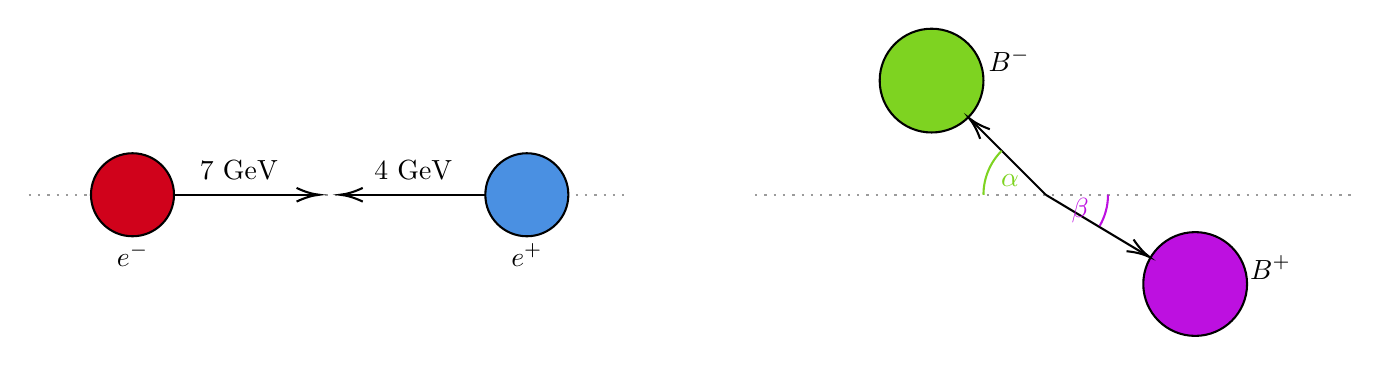
\begin{tikzpicture}[x=0.75pt,y=0.75pt,yscale=-1,xscale=1]
		%uncomment if require: \path (0,300); %set diagram left start at 0, and has height of 300
		
		%Straight Lines [id:da2666196383049946] 
		\draw [color={rgb, 255:red, 155; green, 155; blue, 155 }  ,draw opacity=1 ] [dash pattern={on 0.84pt off 2.51pt}]  (10,90) -- (300,90) ;
		%Shape: Circle [id:dp5941497912321755] 
		\draw  [fill={rgb, 255:red, 208; green, 2; blue, 27 }  ,fill opacity=1 ] (40,90) .. controls (40,78.95) and (48.95,70) .. (60,70) .. controls (71.05,70) and (80,78.95) .. (80,90) .. controls (80,101.05) and (71.05,110) .. (60,110) .. controls (48.95,110) and (40,101.05) .. (40,90) -- cycle ;
		%Shape: Circle [id:dp5300941970691377] 
		\draw  [fill={rgb, 255:red, 74; green, 144; blue, 226 }  ,fill opacity=1 ] (230,90) .. controls (230,78.95) and (238.95,70) .. (250,70) .. controls (261.05,70) and (270,78.95) .. (270,90) .. controls (270,101.05) and (261.05,110) .. (250,110) .. controls (238.95,110) and (230,101.05) .. (230,90) -- cycle ;
		%Straight Lines [id:da791965915355674] 
		\draw    (80,90) -- (148,90) ;
		\draw [shift={(150,90)}, rotate = 180] [color={rgb, 255:red, 0; green, 0; blue, 0 }  ][line width=0.75]    (10.93,-3.29) .. controls (6.95,-1.4) and (3.31,-0.3) .. (0,0) .. controls (3.31,0.3) and (6.95,1.4) .. (10.93,3.29)   ;
		%Straight Lines [id:da5138005195075709] 
		\draw    (230,90) -- (162,90) ;
		\draw [shift={(160,90)}, rotate = 360] [color={rgb, 255:red, 0; green, 0; blue, 0 }  ][line width=0.75]    (10.93,-3.29) .. controls (6.95,-1.4) and (3.31,-0.3) .. (0,0) .. controls (3.31,0.3) and (6.95,1.4) .. (10.93,3.29)   ;
		%Straight Lines [id:da4344549993609035] 
		\draw [color={rgb, 255:red, 155; green, 155; blue, 155 }  ,draw opacity=1 ] [dash pattern={on 0.84pt off 2.51pt}]  (360,90) -- (650,90) ;
		%Shape: Circle [id:dp5014291513295692] 
		\draw  [fill={rgb, 255:red, 126; green, 211; blue, 33 }  ,fill opacity=1 ] (420,35) .. controls (420,21.19) and (431.19,10) .. (445,10) .. controls (458.81,10) and (470,21.19) .. (470,35) .. controls (470,48.81) and (458.81,60) .. (445,60) .. controls (431.19,60) and (420,48.81) .. (420,35) -- cycle ;
		%Shape: Circle [id:dp2010294594289822] 
		\draw  [fill={rgb, 255:red, 189; green, 16; blue, 224 }  ,fill opacity=1 ] (547,133) .. controls (547,119.19) and (558.19,108) .. (572,108) .. controls (585.81,108) and (597,119.19) .. (597,133) .. controls (597,146.81) and (585.81,158) .. (572,158) .. controls (558.19,158) and (547,146.81) .. (547,133) -- cycle ;
		%Straight Lines [id:da9297103902850272] 
		\draw    (500,90) -- (464.41,54.41) ;
		\draw [shift={(463,53)}, rotate = 45] [color={rgb, 255:red, 0; green, 0; blue, 0 }  ][line width=0.75]    (10.93,-3.29) .. controls (6.95,-1.4) and (3.31,-0.3) .. (0,0) .. controls (3.31,0.3) and (6.95,1.4) .. (10.93,3.29)   ;
		%Straight Lines [id:da9786927386703091] 
		\draw    (500,90) -- (548.29,118.97) ;
		\draw [shift={(550,120)}, rotate = 210.96] [color={rgb, 255:red, 0; green, 0; blue, 0 }  ][line width=0.75]    (10.93,-3.29) .. controls (6.95,-1.4) and (3.31,-0.3) .. (0,0) .. controls (3.31,0.3) and (6.95,1.4) .. (10.93,3.29)   ;
		%Shape: Arc [id:dp2642691597839596] 
		\draw  [draw opacity=0] (470,90) .. controls (470,81.72) and (473.36,74.22) .. (478.79,68.79) -- (500,90) -- cycle ; \draw  [color={rgb, 255:red, 126; green, 211; blue, 33 }  ,draw opacity=1 ] (470,90) .. controls (470,81.72) and (473.36,74.22) .. (478.79,68.79) ;  
		%Shape: Arc [id:dp1349982239947891] 
		\draw  [draw opacity=0] (530,90) .. controls (530,90) and (530,90) .. (530,90) .. controls (530,90) and (530,90) .. (530,90) .. controls (530,95.47) and (528.54,100.59) .. (525.99,105) -- (500,90) -- cycle ; \draw  [color={rgb, 255:red, 189; green, 16; blue, 224 }  ,draw opacity=1 ] (530,90) .. controls (530,90) and (530,90) .. (530,90) .. controls (530,90) and (530,90) .. (530,90) .. controls (530,95.47) and (528.54,100.59) .. (525.99,105) ;  
		
		% Text Node
		\draw (51,112) node [anchor=north west][inner sep=0.75pt]   [align=left] {$\displaystyle e^{-}$};
		% Text Node
		\draw (241,112) node [anchor=north west][inner sep=0.75pt]   [align=left] {$\displaystyle e^{+}$};
		% Text Node
		\draw (91,72) node [anchor=north west][inner sep=0.75pt]   [align=left] {7 GeV};
		% Text Node
		\draw (175,72) node [anchor=north west][inner sep=0.75pt]   [align=left] {4 GeV};
		% Text Node
		\draw (477,79) node [anchor=north west][inner sep=0.75pt]  [color={rgb, 255:red, 126; green, 211; blue, 33 }  ,opacity=1 ] [align=left] {$\displaystyle \alpha $};
		% Text Node
		\draw (511,90) node [anchor=north west][inner sep=0.75pt]  [color={rgb, 255:red, 189; green, 16; blue, 224 }  ,opacity=1 ] [align=left] {$\displaystyle \beta $};
		% Text Node
		\draw (471,18) node [anchor=north west][inner sep=0.75pt]   [align=left] {$\displaystyle B^{-}$};
		% Text Node
		\draw (597,118) node [anchor=north west][inner sep=0.75pt]   [align=left] {$\displaystyle B^{+}$};
	\end{tikzpicture}
\end{figure}

\begin{enumerate}
	\item[a)] Tomamos \(c = 1\). Asumiendo que \(YZ\) es el plano de scattering, tenemos
	\begin{equation}
		\begin{pmatrix}
			p^{\mu}_{e^{-}}\\
			p^{\mu}_{e^{+}}\\
			p^{\mu}_{B^{-}}\\
			p^{\mu}_{B^{+}}
		\end{pmatrix} = \begin{pmatrix}
			E_{1} 			& \0 & \0 								& |\vec{p}_{e^{-}}|\\
			E_{2} 			& \0 & \0 								& -|\vec{p}_{e^{+}}|\\
			\mathcal{E}_{1} & \0 & \hfill|\vec{p}_{B^{-}}|\sin\alpha	& -|\vec{p}_{B^{-}}|\cos\alpha\\
			\mathcal{E}_{2} & \0 & -|\vec{p}_{B^{+}}|\sin\beta 		& \hfill|\vec{p}_{B^{+}}|\cos\beta
		\end{pmatrix}
	\end{equation}
	
	De la conservación de 4-momento tendremos:
	\begin{align}
		E_{1} + E_{2} &= \mathcal{E}_{1} + \mathcal{E}_{2} \label{cons_E}\\
		0 &= |\vec{p}_{B^{-}}|\sin\alpha - |\vec{p}_{B^{+}}|\sin\beta \label{cons_py}\\
		|\vec{p}_{e^{-}}| - |\vec{p}_{e^{+}}| &= - |\vec{p}_{B^{-}}|\cos\alpha + |\vec{p}_{B^{+}}|\cos\beta\label{cons_pz}
	\end{align}
	
	De la condición \textit{on-shell}:
	\begin{align}
		E_{1} &\approx |\vec{p}_{e^{-}}| \label{onShell1}\\
		E_{2} &\approx |\vec{p}_{e^{+}}| \label{onShell2}\\
		\mathcal{E}_{1} &= \sqrt{m_{B}^2 + |\vec{p}_{B^{-}}|^2} \label{onShell3}\\
		\mathcal{E}_{2} &= \sqrt{m_{B}^2 + |\vec{p}_{B^{+}}|^2} \label{onShell4}
	\end{align}
	donde \(m_{B}\) es la masa en reposo del bosón \(B\).
	
	De la ec. \ref{cons_E} tenemos
	\begin{equation}
		\mathcal{E}_{2} = E_{1} + E_{2} -\mathcal{E}_{1} \label{E4}
	\end{equation}
	De las condiciones \ref{onShell3} y \ref{onShell4}
	\begin{align}
		|\vec{p}_{B^{-}}|^2 &= \mathcal{E}_{1}^2 - m_{B}^2 \label{p3^2}\\
		|\vec{p}_{B^{+}}|^2 &= \mathcal{E}_{2}^2 - m_{B}^2 \label{p4^2}
	\end{align}
	Y de las condiciones \ref{cons_py} y \ref{cons_pz}:
	\begin{align}
		|\vec{p}_{B^{+}}|\sin\beta &= |\vec{p}_{B^{-}}|\sin\alpha \label{sinBeta} \\
		|\vec{p}_{B^{+}}|\cos\beta &= (|\vec{p}_{e^{-}}| - |\vec{p}_{e^{+}}|) + |\vec{p}_{B^{-}}|\cos\alpha \label{cosBeta}
	\end{align}
	
	Reemplazando las ecs. \ref{onShell1} y \ref{onShell2} en las ecs. \ref{sinBeta} y \ref{cosBeta}, elevándolas al cuadrado y sumándolas:
	\begin{equation}
		|\vec{p}_{B^{+}}|^2 = |\vec{p}_{B^{-}}|^2 + 2(E_{1} - E_{2}) |\vec{p}_{B^{-}}| \cos\alpha + (E_{1} - E_{2})^2
	\end{equation}
	Reemplazando según las ecs. \ref{p3^2} y \ref{p4^2}, y utilizando ec. \ref{E4}:
	\begin{equation}
		(E_{1} + E_{2} -\mathcal{E}_{1} )^2 - m_{B}^2 = \mathcal{E}_{1}^2 - m_{B}^2 + 2(E_{1} - E_{2}) \sqrt{\mathcal{E}_{1}^2 - m_{B}^2} \cos\alpha + (E_{1} - E_{2})^2 \label{eq_E3}
	\end{equation}
	
	Usando Mathematica para resolver la ec. \ref{eq_E3} para \(\mathcal{E}_{1}\) tendremos:
	\begin{equation*}
		\text {FullSimplify}\left[\text{Solve}\left[(E_{1} + E_{2} - \mathcal {E}_{1})^2 - m_{B}^2 = 2\cos (\alpha) (E_{1} - E_{2})\sqrt{\mathcal {E}_{1}^2 - m_{B}^2} + (E_{1} - E_{2})^2 - m_{B}^2 + \mathcal {E}_{1}^2, \mathcal{E}_{1} \right] \right]
	\end{equation*}
	\begin{equation}
		\Rightarrow \mathcal{E}_{1} = \frac {\sqrt {\cos^2 (\alpha) (E_{1} - E_{2})^2\left (4E_{1}^2E_{2}^2 + m_{B}^2\cos^2 (\alpha) (E_{1} - E_{2})^2 - m_{B}^2 (E_{1} + E_{2})^2 \right)} - 2E_{1}E_{2} (E_{1} + E_{2})} {\cos^2 (\alpha) (E_{1} - E_{2})^2 - (E_{1} + E_{2})^2}
	\end{equation}
	Luego, usando la ec. \ref{E4}
	\begin{equation}
		\Rightarrow \mathcal{E}_{2} = E_{1} + E_{2} - \frac {\sqrt {\cos^2 (\alpha) (E_{1} - E_{2})^2\left (4E_{1}^2E_{2}^2 + m_{B}^2\cos^2 (\alpha) (E_{1} - E_{2})^2 - m_{B}^2 (E_{1} + E_{2})^2 \right)} - 2E_{1}E_{2} (E_{1} + E_{2})} {\cos^2 (\alpha) (E_{1} - E_{2})^2 - (E_{1} + E_{2})^2}
	\end{equation}
	
	\item[b)] Tenemos que
	\begin{align}
		s &= \eta (p^{\mu}_{e^{-}} + p^{\mu}_{e^{+}})(p^{\mu}_{e^{-}} + p^{\mu}_{e^{+}})\nonumber \\
		&= (E_{1} + E_{2})^2 - (E_{1} - E_{2})^2 \nonumber\\
		&= 4 E_{1} E{2}\\
		t &= \eta (p^{\mu}_{B^{-}} - p^{\mu}_{e^{-}})(p^{\mu}_{B^{-}} - p^{\mu}_{e^{-}})\nonumber \\
		&= -2E_{1}\cos (\alpha)\sqrt {\mathcal {E}_{1}^2 - m_{B}^2} - 2E_{1}\mathcal{E}_1 + m_{B}^2\\
		u &= 0 + 0 + m_{B}^2 + m_{B}^2 - s - t \nonumber\\
		&= 2E_{1} (\mathcal {E}_{1} - 2E_{2}) + 2E_{1}\cos (\alpha)\sqrt {\mathcal {E}_{1}^2 - m_{B}^2} + m_{B}^2
	\end{align}
\end{enumerate}

\section{Problema 2}
A particle of mass \(m\) and charge \(e\) scatters in the axially symmetric magnetic field which has only \(z\)-component, \(\n{B} = B_z (r) \zhat\), where \(r\) is the distance from axis \(z\), and in what follows we use cylindrical coordinates \((r, \varphi, z)\).

\begin{enumerate}
	\item[a)] Write out explicitly the Lagrangian of this system in cylindrical coordinates. Identify its symmetries, cyclic variables and integrals of motion that may exist in this system.
	
	\item [b)] Demonstrate that it is possible to integrate the equations of motion and find trajectories \(r(t), r(\varphi)\) in general case (for arbitrary \(B_z (r)\)), only using the integrals of motion.
	
	\item[c)] Assume now that the magnetic field vanishes rapidly in the limit \(r\rightarrow\infty\), so the particles move freely at large distances. A charge particle with initial velocity \(\n{v}_0 = v_0 \xhat\) scatters in the above-mentioned magnetic field. Find the general solution (analytic expression) which allows to calculate the scattering angle \(\theta\) as a function of the impact parameter \(\rho\) and velocity \(v_\infty\) in any magnetic field \(B_z (r)\).
	\begin{enumerate}
		\item[i.] Assume that the magnetic vector potential is given by
		\begin{equation*}
			A_\varphi(r) = \left\lbrace \begin{matrix}
				\dfrac{L}{e r}\left(1 - \dfrac{r^2}{R^2}\right), & r < R \vspace{3mm}\\
				0, & r > R
			\end{matrix}\right. , ~~~~~ B_z = \left\lbrace \begin{matrix}
			-\dfrac{2 L}{e R^2}, & r < R \vspace{3mm}\\
			0, & r > R
			\end{matrix}\right.
		\end{equation*}
		Using your general result, find explicitly the scattering angle \(\theta(\rho)\) for the angular momentum \(M_z = L\).
	\end{enumerate}
\end{enumerate}

\begin{enumerate}
	\item[a)] Tenemos la velocidad:
	\begin{equation}
		\n{v} = \dot{r}\rhat + r \dot{\varphi} \phat + z \zhat
	\end{equation}
	Asumiendo que conocemos \(\n{A} = A_\varphi(r) \phat\) tal que \(\n{B} = \ro\n{A}\), el lagrangiano tendrá la forma
	\begin{align}
		L &= \frac{1}{2} m \n{v}^2 + e \n{v}\cdot\n{A}(r) \nonumber\\
		&= \frac{1}{2} m \left(\dot{r}^2 + r^2 \dot{\varphi}^2 + \dot{z}^2\right) + e A_\varphi(r) r \dot{\varphi}
	\end{align}
	De aquí se aprecia que \(\varphi\) y \(z\) son coordenadas cíclicas, por lo que tendremos simetría angular y en el eje \(z\):
	\begin{align}
		Q_\varphi &= \pd{L}{\dot{\varphi}} = m r^2 \dot{\varphi} + e A_\varphi(r) r = \mathrm{const.} \label{Qphi}\\
		Q_z &= \pd{L}{\dot{z}} = m\dot{z} = \mathrm{const.}
	\end{align}
	Y, ya que el tiempo no aparece explícitamente, se conservará la energía:
	\begin{equation}
		E = \frac{1}{2} m \left(\dot{r}^2 + r^2 \dot{\varphi}^2 - \dot{z}^2\right) + e A_\varphi(r) r \dot{\varphi} = \mathrm{const.} \label{E}
	\end{equation}
	
	
	\item[b)] De la ec. \ref{Qphi}, resolviendo para \(\dot{\varphi}\):
	\begin{align}
		\dot{\varphi} &= \frac{Q_\varphi - e r A_\varphi(r)}{m r^2}\\
		\Rightarrow \varphi - \varphi_0 &= \int_{0}^{t} \frac{Q_\varphi - e r A_\varphi(r)}{m r^2} \, dt\nonumber\\
		\varphi(t) - \varphi_0 &= \frac{Q_\varphi - e r A_\varphi(r)}{m r^2} t
	\end{align}
	Y de la ec. \ref{E}:
	\begin{align}
		\dot{r}^2 &= \frac{2}{m}(E - e A_\varphi(r) r \dot{\varphi}) - r^2 \dot{\varphi}^2 - \dot{z}^2\nonumber\\
		&= \frac{1}{m} \left(2 E - \frac{Q_z^2}{m} - \frac{(Q_\varphi - e r A_\varphi(r))^2}{m r^2}\right)\nonumber\\
		\Rightarrow \dot{r} &= \sqrt{\frac{1}{m} \left(2 E - \frac{Q_z^2}{m} - \frac{(Q_\varphi - e r A_\varphi(r))^2}{m r^2}\right)}
	\end{align}
	Por lo que
	\begin{equation}
		\Rightarrow t - t_0 = \int_{r_0}^{r} \sqrt{\frac{1}{m} \left(2 E - \frac{Q_z^2}{m} - \frac{(Q_\varphi - e r A_\varphi(r))^2}{m r^2}\right)}\, dr
	\end{equation}
	Y, para \(r(\varphi)\):
	\begin{align}
		\td{r}{\varphi} &= \frac{\dot{r}}{\dot{\varphi}} = \frac{m \dot{r} r^2}{Q_\varphi - e r A_\varphi(r)} \nonumber\\
		\Rightarrow \varphi - \varphi_0 &= \int_{r_0}^{r} \frac{Q_\varphi - e r A_\varphi(r)} {m r^2} \frac{1}{\sqrt{\frac{1}{m} \left(2 E - \frac{Q_z^2}{m} - \frac{(Q_\varphi - e r A_\varphi(r))^2}{m r^2}\right)}} \, dr \label{phi(r)}
	\end{align}
	En ambos casos tenemos expresiones para \(r(t)\) y \(r(\varphi)\) que dependen solo de la forma de \(A_\varphi\) y de constantes de movimiento.

	\item[c)] A una distancia infinitamente grande de la región de potencial tendremos que
	\begin{equation}
		E = \frac{1}{2} m v_0^2
	\end{equation}
	Y, además, como la velocidad inicial se encuentra solo en el eje \(x\):
	\begin{equation}
		Q_z = m\dot{z} = 0
	\end{equation}
	Y, finalmente, en una región alejada donde \(A_\varphi = 0\), tenemos el resultado típico:
	\begin{align}
		Q_\varphi &= m \rho^2 \dot{\varphi} + 0 \nonumber\\
		&= m v_0 \rho
	\end{align}
	
	Ahora, tomando la ec. \ref{phi(r)}
	\begin{align}
		\varphi - \varphi_0 &= \int_{r_0}^{r} \frac{Q_\varphi - e r A_\varphi(r)} {m r^2} \frac{1}{\sqrt{\frac{1}{m} \left(2 E - \frac{Q_z^2}{m} - \frac{(Q_\varphi - e r A_\varphi(r))^2}{m r^2}\right)}} \, dr \nonumber\\
		\varphi - \varphi_0 &= \int_{r_0}^{r} \frac{m v_0 \rho - e r A_\varphi(r)} {m r^2} \frac{1}{\sqrt{\frac{1}{m} \left(m v_0^2- \frac{(m v_0 \rho - e r A_\varphi(r))^2}{m r^2}\right)}} \, dr\nonumber\\
		\varphi - \varphi_0 &= \int_{r_0}^{r} \frac{m v_0 \rho - e r A_\varphi(r)}{r \sqrt{m^2 v_0^2 r^2  - (m v_0 \rho - e r A_\varphi(r))^2}} \, dr
	\end{align}
	
	El rango completo de la coordenada angular \(\Delta \varphi\) vendrá de integrar en \([r_\mathrm{min}, \infty]\), donde \(r_\mathrm{min}\) es la distancia más cercana al centro del campo, es decir:
	\begin{equation}
		\Delta \varphi = 2\int_{r_\mathrm{min}}^{\infty} \frac{m v_0 \rho - e r A_\varphi(r)}{r \sqrt{m^2 v_0^2 r^2  - (m v_0 \rho - e r A_\varphi(r))^2}} \, dr
	\end{equation}
	Y, ya que \(\theta = \pi - 2\Delta\varphi\)
	\begin{equation}
		\theta(\rho, v_\infty) =  \pi - 2\int_{r_\mathrm{min}}^{\infty} \frac{m v_0 \rho - e r A_\varphi(r)}{r \sqrt{m^2 v_0^2 r^2  - (m v_0 \rho - e r A_\varphi(r))^2}} \, dr
	\end{equation}
	\begin{enumerate}
		\item[i.] Considerando
		\begin{equation}
			A_\varphi(r) = \left\lbrace \begin{matrix}
				\dfrac{L}{e r}\left(1 - \dfrac{r^2}{R^2}\right), & r < R \vspace{3mm}\\
				0, & r > R
			\end{matrix}\right.
		\end{equation}
		donde
		\begin{equation}
			L = Q_\varphi = m v_0 \rho
		\end{equation}
		Tendremos que
		\begin{equation}
			\theta(\rho, v_\infty) =  \pi - 2\int_{r_\mathrm{min}}^{R} \frac{L - e r A_\varphi(r)}{r \sqrt{(m v_0 r)^2 - (L - e r A_\varphi(r))^2}} \, dr - 2\int_{R}^{\infty} \frac{L}{r \sqrt{(m v_0 r)^2  - L^2}} \, dr
		\end{equation}
		La primera integral, usando Mathematica:
		\begin{align}
			&\int_{r_\mathrm{min}}^{R} \frac{m v_0 \rho - e r A_\varphi(r)}{r \sqrt{m^2 v_0^2 r^2  - (m v_0 \rho - e r A_\varphi(r))^2}} \, dr \nonumber\\
			=& L \int_{r_\mathrm{min}}^{R} \frac{\left(1 - \dfrac{r^2}{R^2}\right)}{r \sqrt{m^2 v_0^2 r^2  - \left(1 - \dfrac{r^2}{R^2}\right)^2}} \, dr \nonumber\\
			=& \arcsin\left(\frac{m v_0 r}{R L}\right)
		\end{align}
		
		La segunda integral, usando Mathematica y \texttt{FullSimplify}:
		\begin{equation}
			\int_{R}^{\infty} \frac{m v_0 \rho}{r \sqrt{(m v_0 r)^2  - (m v_0 \rho)^2}} \, dr = - \arcsin\left(\frac{\rho}{R}\right)
		\end{equation}
		
		Finalmente,
		\begin{equation}
			\theta(\rho, v_\infty) =  \pi - 2 \arcsin\left(\frac{m v_0 r}{R L}\right) +  2 \arcsin\left(\frac{\rho}{R}\right)
		\end{equation}
	\end{enumerate}
\end{enumerate}


























\end{document}